%-------------------------------------------------------------------------------
% seq66_sessions
%-------------------------------------------------------------------------------
%
% \file        seq66_sessions.tex
% \library     Documents
% \author      Chris Ahlstrom
% \date        2020-10-03
% \update      2020-10-12
% \version     $Revision$
% \license     $XPC_GPL_LICENSE$
%
%  Provides a discussion of how Seq66 supports session management, specifically
%  the Non Session Manager.
%
%-------------------------------------------------------------------------------

\section{Seq66 Session Management}
\label{sec:sessions}

   \textsl{Seq66} supports session management in three ways:

   \begin{enumber}
      \item \textbf{Non Session Manager}
      \item \textbf{Signals}
      \item \textbf{LASH}
   \end{enumber}

%  See \sectionref{subsec:seq66_rc_file_midi_control},

\subsection{Seq66 Session Management / NSM}
\label{subsec:sessions_nsm}

   \index{sessions!nsm}
   NSM support is well underway, but still in progress.
   The first thing to do for session management is make sure that the
   application is capable of various levels of session management, from none to
   a full-blown session manager like the \textsl{Non Session Manager}.  The
   basic session management consist of being able to properly start the
   application and let it run properly during its life-cyle, whether it is a
   command-line application or a graphical application.

\subsubsection{Seq66 Session Management / NSM / First Run Before Using NSM}
\label{subsec:sessions_nsm_before_using_nsm}

   It is important, after installing \textsl{Seq66}, to run it normally. This
   action creates the default configuration files in
   \texttt{/home/user/.config/seq66}:

\begin{verbatim}
   nsm $ qseq66 
   [No 'rc' file, will create: qseq66.rc/ctrl/midi/mutes/drums/playlist]
   [No 'usr' file, will create: /home/user/.config/seq66/qseq66.usr]
   [File exists: /home/user/.config/seq66/qseq66.rc]
   [Saving initial config files to session directory!]
   [Writing 'rc': /home/user/.config/seq66/qseq66.rc]
   [Writing 'ctrl': /home/user/.config/seq66/qseq66.ctrl]
   [Writing 'mutes': /home/user/.config/seq66/qseq66.mutes]
   [Writing 'usr': /home/user/.config/seq66/qseq66.usr]
   . . .
\end{verbatim}

   There will be some unimportant errors due to JACK not running or an
   inability to open a play-list or drums file, but they can be ignored.
   Then exit \textsl{Seq66} to ensure the configuration files are ready.
   The \texttt{qseq66.usr} file can then be edited to allow \textsl{Seq66} to
   use NSM.  Look for the following lines in that file:

\begin{verbatim}
   [user-session]
   session = none
\end{verbatim}

   It is then important to change the "session" line to

\begin{verbatim}
   session = nsm
\end{verbatim}

   Now we are ready to run the Non Session Manager, as described in the next
   section.  However, note that \texttt{qseq66} can still be run outside of a
   session manager.  It will detect the absense of the session manager and run
   normally.

\subsubsection{Seq66 Session Management / NSM / First Run}
\label{subsec:sessions_nsm}

   Now that we have the initial configuration, we want to run \textsl{Seq66}
   under NSM and create a configuration in the \texttt{NSM Sessions} directory.
   For illustration, we run \textsl{NSM} from a terminal window, which can be
   very helpful when problems occur.

\begin{verbatim}
   $ non-session-manager
   [non-session-manager] Starting daemon...
   [nsmd] Session root is: /home/user/NSM Sessions
   NSM_URL=osc.udp://mlsasus.mls:19625/
   [nsmd] Listing sessions
\end{verbatim}

   \index{sessions!non-starter}
   If \textsl{NSM} refuses to start, make sure that the \texttt{liblo} library
   from the OSC project is installed.  If it is installed, then check the
   \texttt{/etc/hosts} file to make sure that the loopback interfaces are
   defined:

\begin{verbatim}
   127.0.0.1   localhost
   127.0.1.1   mlsasus.mls mlsasus
\end{verbatim}

   The NSM user-interface (not shown here) that comes up is empty at first.  So
   we now create a session by clicking the NSM \textsl{New} button, and
   entering a session name (e.g. "Seq66") in the prompt that comes up.  We see,
   in the console window, a couple of "/nsm/server/new" \textsl{OSC} messages
   about the creation of the session.

\begin{verbatim}
   [non-session-manager] Sending new for: Seq66
   [nsmd] Creating new session "Seq66"
   [non-session-manager] /nsm/server/new says Created.
   [non-session-manager] /nsm/server/new says Session created
\end{verbatim}

   Next, we click the \textsl{Add Client to Session}, and, since
   \texttt{qseq66} has been installed, it is in the "PATH" and its executable
   name can be entered simply: "qseq66".  A number of console messages from
   \textsl{Seq66} appear, plus some messages from \textsl{NSM}:

\begin{verbatim}
	[non-session-manager] Sending add for: qseq66
	[nsmd] Process has pid: 2797436
	[nsmd] Launching qseq66
	[nsmd] Got announce from seq66
	[nsmd] Client was expected.
	[nsmd] Process has pid: 2797436
	[nsmd] The client "seq66" at "osc.udp://127.0.0.1:13318/" informs us it's
    ready to receive commands.
\end{verbatim}

	Once \textsl{Seq66} is running under \textsl{NSM}, we can see what has
   been created to support the session.  The directory that \textsl{NSM}
   creates by default is \texttt{/home/user/NSM Sessions}.

\begin{verbatim}
   $ pwd
   /home/user/NSM Sessions
   $ ls -RF
	.:
		Seq66/
	./Seq66:
		seq66.nIRJI/  session.nsm
	./Seq66/seq66.nIRJI:
		config/  midi/
	./Seq66/seq66.nIRJI/config:
		qseq66.ctrl  qseq66.mutes  qseq66.rc  qseq66.usr
	./Seq66/seq66.nIRJI/midi: <empty>
\end{verbatim}

	So \textsl{NSM} has created a directory with the session name we gave it:
   \texttt{Seq66}.  Under that directory is a file, \texttt{session.nsm}, which
   contains information like the following when we click the \textsl{Save}
   button in the \textsl{NSM} user-interface:

\begin{verbatim}
   seq66:qseq66:nIRJI
\end{verbatim}

   The format of line is "appname:exename:nXXXX".

   Also created is a directory, \texttt{seq66.nIRJI}, which is the root of the
   \texttt{Seq66} session.  The "IRJI" portion is randomly generated by
   \textsl{NSM}.

   The rest of the directories are generated by \textsl{Seq66}, which creates
   new \texttt{config} directory (to be used instead of
   \texttt{/home/user/.config/seq66}) and a \texttt{midi} directory which will
   contain any new or imported MIDI files.  The new \texttt{config} directory
   contains versions of the various configuration files that will always be
   used to start up \textsl{Seq66} during the session.  One can also add valid
   play-list and drums files to that directory.

\subsubsection{Seq66 Session Management / Sessions Tab}
\label{subsubsec:sessions_ui}

   A new user-interface, the "Session" tab, is provided to orient the user to
   the setup supported by the session.

\begin{figure}[H]
   \centering 
   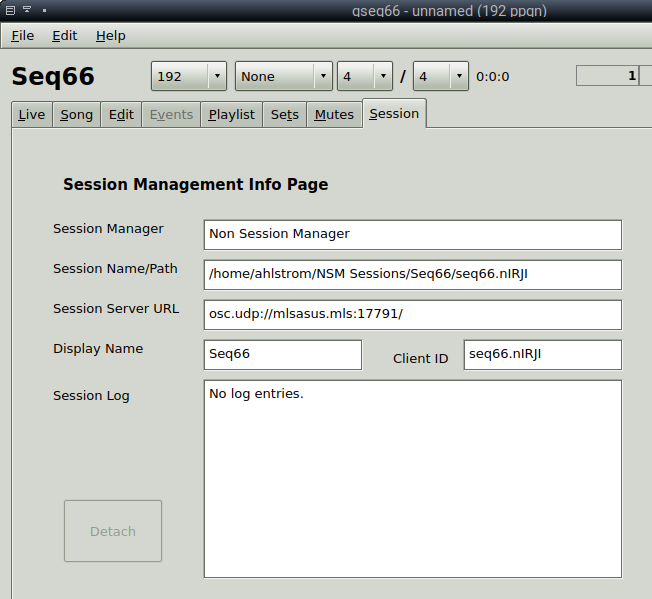
\includegraphics[scale=0.65]{sessions/qseq66-session-tab.png}
   \caption*{Session Tab When Running Under NSM}
\end{figure}

   \index{sessions!ui}
   This section describes the \textsl{Session} tab in the main
   \textsl{Seq66} window.  At present, this tab is just informative.  It
   displays the following bits of information that \textsl{Seq66} has received
   from \textsl{NSM} via the \texttt{nmsd} daemon:

   \begin{itemize}
      \item Name of the session manager.
      \item Session path for the session, the root directory of the session.
         All data goes into this directory.
      \item The OSC URL of the session, which includes the port number.
         Generally, the port number is selected at run-time, but it is also
         possible to configure \textsl{NSM} to use a specific port number.
      \item Display-name for the session.
      \item The generated client ID for the session.
      \item The log of action of the session manager. Not yet supported.
   \end{itemize}

   The \textsl{Detach} is disabled because this feature is not ready.

\subsubsection{Seq66 Session Management / File Menu}
\label{subsubsec:sessions_file_menu}

   The author of \textsl{NSM} has provided documentation for session-management
   which provides very strict instructions on how an application must behave
   under session management.  \textsl{Seq66} tries very hard to stick to these
   instructions.  One major adjustment an application must make is to adhere to
   the "File menu" guidelines.

\begin{figure}[H]
   \centering 
   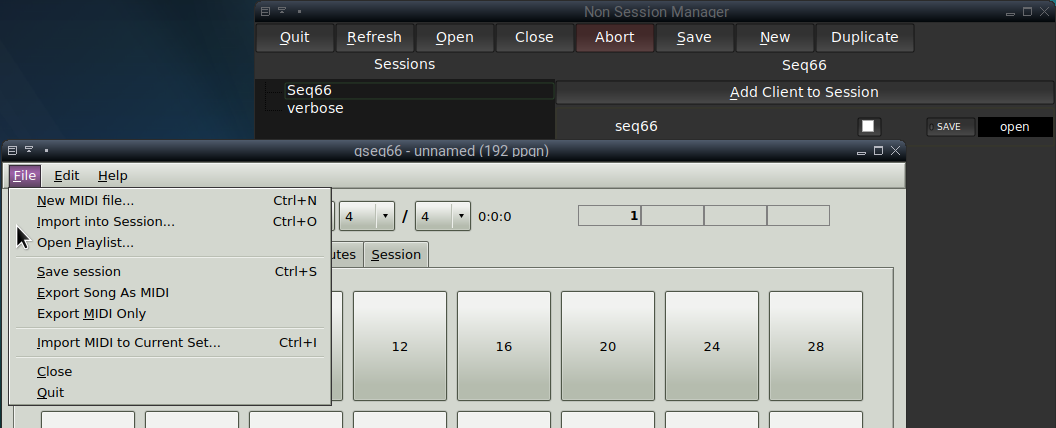
\includegraphics[scale=0.65]{sessions/nsm-qseq66-menus.png}
   \caption*{File Menu When Running Under NSM}
\end{figure}

   The following items describe the menu entries.  Some of these are still in
   progress or still need to be enforced.

   \begin{itemize}
      \item \textbf{New MIDI File}.
         This function prompts for the name of a
         new MIDI file and clears the current MIDI file.  The file-name must not
         include a full-path to the file.  The path is hardwired by the
         session.  A relative path can be included.  This name is needed
         because there is no "Save As" option when running in an \textsl{NSM}
         session.
      \item \textbf{Import into Session}.
         Prompts the user for a MIDI file to
         be imported (copied) into the current session.  The path to the file
         is then adjusted to use the \textsl{NSM} \texttt{midi} subdirectory.
      \item \textbf{Open Playlist}.
         Works the same as without session
         management, but gets the list from the session directory.
         TODO: STILL IN PROGRESS.
      \item \textbf{Save Session}.
         This function saves the main configuration
         files (except for the 'usr' file), saves the play-list and note-mapper
         files, if in use, and saves the current MIDI file, if any.
      \item \textbf{Export Song As MIDI}.
         Allows exporting the current song as a stock MIDI file, using the
         performance information (triggers) to write the MIDI data as it would
         be played in "song" mode.
         TODO: IS THE DEFAULT DIRECTORY the current session???
      \item \textbf{Export MIDI Only}.
         Allows exporting the current song as a stock MIDI file.
         The "proprietary" SeqSpec data is \textsl{not} written.
         TODO: IS THE DEFAULT DIRECTORY the current session???
      \item \textbf{Import MIDI to Current Set}.
         This item allows the user to grab a MIDI file from anywhere and import
         it into the current set.
      \item \textbf{Close}.
         Allows \textsl{Seq66} to detach from session management.
         TODO:  should save the session and close the session.
         NEEDS MORE THOUGHT.
      \item \textbf{Quit}.
         Quits \textsl{Seq66}.
         TODO: NEED TO INFORM NSM WE ARE QUITTING!!!!!!
   \end{itemize}

\subsection{Seq66 Session Management / Signals}
\label{subsec:sessions_signals}

   \index{sessions!signals}
   By default, the basic form of session management in
   \textsl{Seq66} occurs by signals.  A
   session manager can start \textsl{Seq66}, and it can tell \textsl{Seq66} to
   save or stop.  Starting is done by a system call to spawn the application.
   The save and stop actions are supported by sending the following signals to
   the application:

   \begin{itemize}
      \item \texttt{SIGINT}.
         This signal stops \textsl{Seq66}. It corresponds
         to using \texttt{Ctrl-C} from the command-line to stop \textsl{Seq66}.
         This signal should work for both the graphical and command-line
         application.  As \textsl{Seq66} shuts down, it does its normal saving
         of the current state of the configuration.
      \item \texttt{SIGTERM}.
         This signal also stops \textsl{Seq66}.  It can
         be sent by an application to exit \textsl{Seq66}.
      \item \texttt{SIGUSR1}.
         This signal tells \textsl{Seq66} to save.  This
         action will save the current MIDI file.
   \end{itemize}

   One application that can control \textsl{Seq66}, to some extent, when not in
   session mode, is \textsl{nsm-proxy}:

      \url{https://non.tuxfamily.org/wiki/nsm-proxy}

   \textsl{NSM-Proxy} is a simple \textsl{NSM} client for wrapping non-NSM
   capable programs. It enables the use of programs supporting LADISH Level 0
   and 1, and programs which accept their configuration via command-line
   arguments.  There is a command-line version and a graphical version.

   MORE TO COME on how to use nsm-proxy.

\subsection{Seq66 Session Management / LASH}
\label{subsec:sessions_lash}

   \index{sessions!lash}
   MORE TO COME.
   LASH support has not yet been fully reimplemented and retested.

%-------------------------------------------------------------------------------
% vim: ts=3 sw=3 et ft=tex
%-------------------------------------------------------------------------------
